\section{KPMG on ERP Systems}\label{technical-presentation}

\subsection{Introduction and Agenda}\label{introduction-and-agenda}

\begin{figure}[!h]
    \centering
    \includegraphics[page=2, trim = 2cm 7cm 2cm 0cm, clip, width=\textwidth]{images/01 - KPMG_IT Advisory Services_ENG_v1.pdf}
\end{figure}

We have plenty of time this morning, so let's make the most of it. I
propose structuring the next 60 minutes as follows:

First, I will provide a brief introduction about myself and the company
I work for. Then, we will dive into the documentation I have prepared.

To begin, my name is Marco Trammelli, and I am a senior manager of advisory at the KPMG company. I will give you an overview of the system we
will be discussing today, whic  h serves as a prerequisite for
understanding the rest of the session.

Next, we will move on to the second part of today's session, where I
will introduce a test case scenario that you will be working on in the
coming days. After that, I will hand over the stage to my colleague from
the HR department.

\subsection{System Overview}\label{system-overview}

\subsubsection{Historical Perspective and
    Evolution}\label{historical-perspective-and-evolution}

Let's start with a brief introduction to the system, considering its
historical perspective and evolution. We'll also provide an overview of
a sample system, the SAP ERP system, which is widely used in the
market. If time permits, we'll then move on to our recommendations for
implementation and development projects.

\begin{figure}[!h]
    \centering
    \includegraphics[page=3, trim = 2cm 5cm 1cm 0cm, clip, width=\textwidth]{images/01 - KPMG_IT Advisory Services_ENG_v1.pdf}
\end{figure}

The term ``legacy system'' refers to a collection of autonomous
applications, each with its own database. These systems are not
interconnected, and interfaces need to be developed and implemented to
establish communication between them. In the following roadmap, we'll
highlight the evolution of these systems over the decades, starting from
the first enterprise resource planning system in the 1970s.

\subsubsection{Legacy Systems vs.~ERP
    Systems}\label{legacy-systems-vs.-erp-systems}

\begin{figure}[!h]
    \centering
    \includegraphics[page=4, trim = 2cm 3cm 1cm 0cm, clip, width=\textwidth]{images/01 - KPMG_IT Advisory Services_ENG_v1.pdf}
\end{figure}

Basically, this system was initially developed for manufacturing and
production processes within the organization. Over time, additional
features were added to support other functions and processes. This
evolution led to what we now call the extended ERP system.

\begin{figure}[!h]
    \centering
    \includegraphics[page=5, trim = 2cm 3cm 2cm 0cm, clip, width=\textwidth]{images/01 - KPMG_IT Advisory Services_ENG_v1.pdf}
\end{figure}

Now, let's briefly compare legacy systems with ERP systems. Legacy
systems are often referred to as closed systems. They store information
about past actions in their own databases. Each function in the
organization, such as purchasing, shipping, production, warehouse
administration, and sales, typically has its own separate system. This
lack of a common repository can lead to duplicated activities and
operational inconsistencies across different business functions.

\begin{figure}[!h]
    \centering
    \includegraphics[page=9, trim = 2cm 2.5cm 2cm 0cm, clip, width=\textwidth]{images/01 - KPMG_IT Advisory Services_ENG_v1.pdf}
\end{figure}

On the other hand, the ERP system is a
unique system that can simulate and propose future scenarios instead of
focusing on the past. This system shares a common database, which I will
refer to as a table or database. Additionally, there is a sharing of
operational logic among different functional areas within a company,
such as purchasing, shipping, and production. Each block in this diagram
represents a specific function within the organization. It is important
to note the close interconnection of activities carried out in these
functional areas. Instead of developing separate programs for each
function, the system allows for the development of shared programs for
multiple functions. These key features cover various business processes,
including logistics, accounting, production, and human resources. These
processes are supported by a set of application elements known as
modules. Throughout this presentation, we will explore how each module
represents a specific function within the organization.

\begin{figure}[!h]
    \centering
    \includegraphics[page=18, trim = 2cm 4cm 2cm 0cm, clip, width=\textwidth]{images/01 - KPMG_IT Advisory Services_ENG_v1.pdf}
\end{figure}

Can someone explain what a legacy system is and what the main
differences are between a legacy system and an ERP system? Let's imagine a
company and focus on the purchase processes, such as purchase
requisitions, purchase orders, receiving invoices, etc. Invoicing is
related to accounting and finance, while purchasing is mainly related to
the buyer or someone in the purchasing department. It's not interesting
to discuss the connection between finance and accounting in these
processes. A legacy system uses different tables that need to be
reconciled, requiring the implementation of multiple interfaces and
effort to check for redundant data. On the other hand, an ERP system has
a common structure with a unique table, eliminating the need for
reconciliation and interfaces. By implementing an ERP system from the
beginning, an organization can focus on developing efficiency in
processes instead of spending time and money on reconciling data. Legacy
systems are difficult to integrate with external tools, while ERP
systems already have connections in place. ERP systems also come with
embedded best practices for accounting, finance, and purchasing
processes, making them ready to use with just configuration based on the
organization's specificity. Legacy systems require specific interfaces
to integrate with other software and require the organization to align
with best practices. If a specific process is not in line with best
practices, it cannot be included in an ERP system without revising and
adapting it. When selecting an ERP system, industry specificity,
specific organizational issues, business strategy, industrial
development plans, processes, and resources should be considered. These
factors will guide the software selection process, whether it involves
implementing an ERP system from the market or looking for specific
software applications from local vendors.

\subsubsection{ERP Implementation and
    Development}\label{erp-implementation-and-development}

\begin{figure}[!h]
    \centering
    \includegraphics[page=8, trim = 2cm 5cm 2cm 0cm, clip, width=\textwidth]{images/01 - KPMG_IT Advisory Services_ENG_v1.pdf}
\end{figure}

The logistics department, accounting, production, sales, and human
resources all benefit from the adoption of an ERP system. By sharing the
same repository and database, businesses can ensure the uniqueness and
universality of their data and business information. Major software
vendors like Microsoft and SAP produce and release ERP systems, such as
MRP (Material Requirements Planning).

From a technical perspective, ERP systems use a relational database and
operate on a client-server architecture. They also offer vertical
solutions tailored to specific industries, such as automotive or
healthcare, which have unique business processes and requirements.

Implementing an ERP system allows companies to leverage best practices
and standardized processes across departments, eliminating the need to
reinvent the wheel for each company. This saves time and resources while
ensuring efficiency and consistency.

Moving forward, many companies are already using ERP systems like
Microsoft or SAP, but they continue to seek improvements and
enhancements to their systems.

\subsubsection{Future Directions and Cloud
    Computing}\label{future-directions-and-cloud-computing}

\begin{figure}[!h]
    \centering
    \includegraphics[page=12, trim = 2cm 3cm 2cm 0cm, clip, width=\textwidth]{images/01 - KPMG_IT Advisory Services_ENG_v1.pdf}
\end{figure}

In recent years, there have been common words and concepts that have
gained popularity, such as cloud computing and mobility. As a consulting
firm, our clients are increasingly requesting these features to enhance
their processes and handle larger volumes of data. This includes
leveraging analytics and exploring the Internet of Things.

\begin{figure}[!h]
    \centering
    \includegraphics[page=14, trim = 2cm 5cm 2cm 0cm, clip, width=\textwidth]{images/01 - KPMG_IT Advisory Services_ENG_v1.pdf}
\end{figure}

These are the keywords that define the evolution of the
market: accessibility, collaboration, and synchronization are the
driving forces behind this shift. One of the leading software vendors in
this field is SAP, an international company that has been instrumental
in shaping this framework. Until about five years ago, most companies
were developing and implementing their systems on-premise. This meant
that they purchased licenses and installed the software on their own
servers.

Nowadays, many vendors, including SAP, are adopting a philosophy of
moving everything to the cloud. This means that companies looking to
implement SAP solutions no longer need to install them on their own
servers. Instead, everything is accessible through the cloud. The core
business processes, such as finance and accounting, can still be kept
on-premises using the core ERP system. However, specific processes, like
purchasing, can be linked to dedicated cloud solutions.

For instance, consider the purchasing processes of creating a purchase request, issuing a purchase order, and receiving goods. These processes can be efficiently managed using a dedicated cloud solution called Ariba\footnotemark{}, which is tightly integrated with the core ERP system. This is the direction the market is moving towards, and it is important to consider this when making a business case.

In summary, the trend is to move towards cloud-based solutions, with
core processes remaining on-premises and specific processes being
managed through dedicated cloud solutions.

\footnotetext{Ariba is a cloud-based procurement management solution provided by SAP. It integrates with the core ERP system to automate complex workflows, making it easier for employees to search for goods and services, collaborate with suppliers, and manage approvals and invoices \href{https://learning.sap.com/products/intelligent-spend-management/ariba/procurement}{Source 1}.}


\subsection{Integration Challenges and
    Strategies}\label{integration-challenges-and-strategies}

\subsubsection{Choice of an ERP}
\begin{figure}[!h]
    \centering
    \includegraphics[page=22, trim = 2cm 3cm 2cm 0cm, clip, width=\textwidth]{images/01 - KPMG_IT Advisory Services_ENG_v1.pdf}
\end{figure}

\begin{figure}[!h]
    \centering
    \includegraphics[page=23, trim = 1cm 3cm 1cm 0cm, clip, width=\textwidth]{images/01 - KPMG_IT Advisory Services_ENG_v1.pdf}
\end{figure}

In terms of the main software vendor for the ERP there are Oracle and SAP, but first there are some keywords that are important to consider. The structure of the
software is based on modules, with each module representing a specific
area, department, or process. For example, there are modules for the
financial department, controlling, sales, purchasing, and production.
Each module is connected to the others, meaning that actions in one module
can impact other modules. For instance, creating a purchase requisition
or order in the purchasing module may require entering financial objects
that are key elements in the controlling or finance modules.

\subsubsection{ERP Projects}

\begin{figure}[!h]
    \centering
    \includegraphics[page=38, trim = 2cm 2.5cm 2cm 0cm, clip, width=\textwidth]{images/01 - KPMG_IT Advisory Services_ENG_v1.pdf}
\end{figure}

Implementing an ERP system involves three key dimensions: technology,
processes, and people. There are several risks associated with ERP
projects, as shown by the results of previous campaigns. Project
management is crucial, as a poorly structured project plan can lead to
issues. Setting clear business objectives from the beginning is
essential to manage expectations and measure the benefits of the
implementation. Managing complexity and making the right software
selection are also important factors.

When starting a project, it is necessary to collect functional
requirements by interviewing process owners and key users from each
department. These requirements need to be translated into the language
of the ERP system to proceed with the implementation. The implementation
process includes system setup, testing in a quality environment, user
acceptance testing, and training for all users in the company.

\begin{figure}[!h]
    \centering
    \includegraphics[page=39, trim = 2cm 4cm 2cm 0cm, clip, width=\textwidth]{images/01 - KPMG_IT Advisory Services_ENG_v1.pdf}
\end{figure}

Choosing the right software and implementing it can be complex.
Consulting companies often have their own approach and tools to
accelerate the process. It is important to consider the business needs
and plan for the future when selecting and implementing an ERP system.

\begin{figure}[!h]
    \centering
    \includegraphics[page=48, trim = 2cm 1.5cm 2cm 0cm, clip, width=\textwidth]{images/01 - KPMG_IT Advisory Services_ENG_v1.pdf}
\end{figure}

\begin{figure}[!h]
    \centering
    \includegraphics[page=53, trim = 1cm 1.5cm 1cm 0cm, clip, width=\textwidth]{images/01 - KPMG_IT Advisory Services_ENG_v1.pdf}
\end{figure}

In terms of transformation projects, change management is crucial. It
involves explaining the benefits and changes to the organization and its
departments. This includes cost savings and potential revenue increases.
It is important to consider the current state of the legacy system and
its ability to manage processes. If acquiring another company,
integration planning is necessary, whether it involves adopting their
system or finding a common system. The selection of software depends on
specific requirements and constraints, such as supporting collaboration
with suppliers. The relationship between processes, technology, and
change management is essential. In the case of a global company,
localization requirements and multiple instances may need to be
considered. The integration of acquired companies and their IT landscape
is also a strategic consideration.